\namedsection{Architektur des Gesamtsystems} {T}

Die Abbildung \ref{fig:Architektur des Gesamtsystems} veranschaulicht die Architektur des Gesamtsystems unserer Lösung. Dabei wurden die Services im API Management Layer von unserem Team für Statistance entwickelt, welches auf die Drittsysteme der Kunden zugreifen (Customer Systems Layer) und die Daten in der zentralen Datenbank (API Management Layer) speichern. Die Integration der Systeme von Statistance (Frontend und Statistance API Layer) wird über das API Gateway hergestellt, welches REST APIs anbietet und die Anfrage an die entsprechenden Konnektoren weiterleitet, um gewünschte Aktionen (lesen/schreiben) auszuführen. Im Wesentlichen wird die Skalierung/Erweiterbarkeit durch eine flexible Microservice-Architektur erreicht, wobei ein Konnektor autark ist und für ein Drittsystem beim Kunden zuständig ist. Diese und alle weiteren Services im API Management Layer werden dabei zentral über ein Configuration Management Service (Consul) konfiguriert, sodass die Konfiguration der verschiedenen Services leicht verwaltet werden können. Bei zunehmender Skalierung und steigenden Anforderungen, hatten wir für den späteren Verlauf noch weitere Services vorgesehen. So könnten beispielsweise ein Meta Data Repository Service für die Validierung von Input/Output im System, ein Connector Repository Service für die Verwaltung der einzelnen Konnektoren mit eingeführt werden, um weitere Funktionalitäten im System zu unterstützen.

\begin{figure}[!h]
\centering
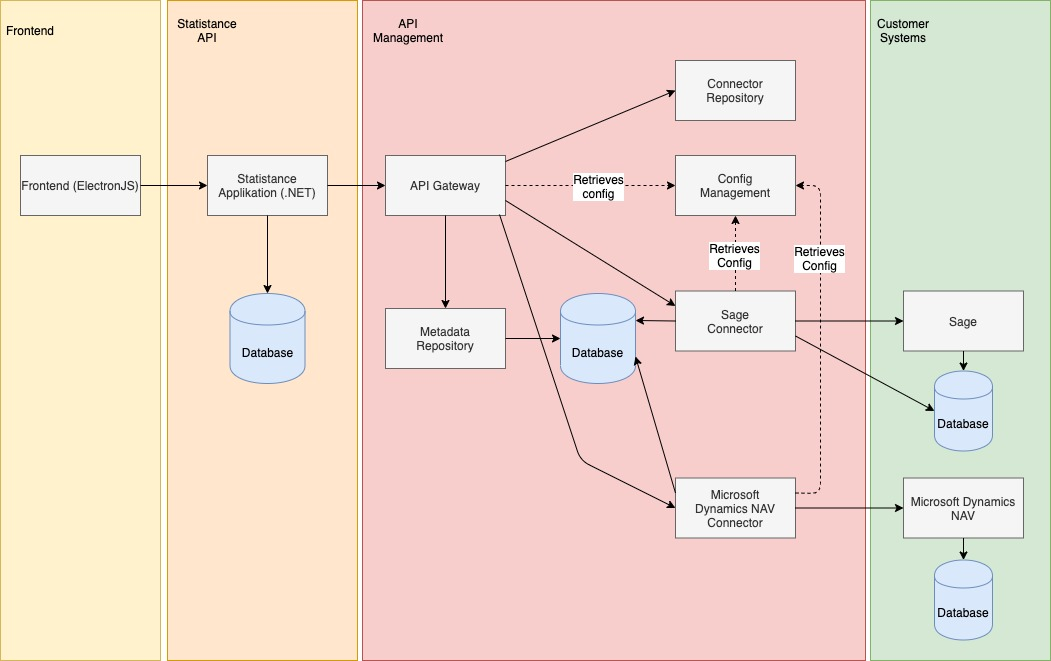
\includegraphics[width=15cm]{images/00_software_architecture/01_Architecture_Overview/architecture_overview.jpg}
\caption{Architektur des Gesamtsystems}
\label{fig:Architektur des Gesamtsystems}
\end{figure}

Die Tabelle \ref{tab:Komponenten und Services im System} listet die Komponenten/Services mit deren Funktion im System auf.

\begin{table}[h!]
\begin{tabular}{|c|p{10cm} |}
\hline
\textbf{Komponente} & \textbf{Beschreibung}\\ \hline \bottomrule
Frontend & • Bietet Zugriff auf die Statistance-Applikation über eine Benutzeroberfläche \newline
•	Wird von Statistance entwickelt \\ \hline
Statistance Application & •	Applikation für statistische Berechnungen \newline
•	Wird von Statistance entwickelt  \\ \hline
Datenbank für die Statistance Application & •	Enthält alle notwendigen Daten für die statische Berechnungen in der Statistance-Applikation \newline
•	Wird von Statistance betrieben und verwaltet \\ \hline
API Gateway & •	Fungiert als zentraler Endpunkt für die Anfragen im API Management Layer \\ \hline
MongoDB & •	Enthält Kundendaten aus Drittsystemen in geeigneter Form nach vordefiniertem Format \newline •	Enthält Daten für API Management \\ \hline
Config Repository & •	Enthält und verwaltet die Konfiguration der einzelnen Services für das API Management \\ \hline
Sage Connector & •	Ist zuständig für die Interaktion mit dem Sage ERP-System \\ \hline
Microsoft Dynamics NAV Connector & •	Ist zuständig für die Interaktion mit Microsoft Dynamics NAV \\ \hline
Connector Repository & •	Verwaltet die verfügbaren Konnektoren im System \\ \hline
Meta Data Repository & •	Enthält Metadaten, Schemata für die Validierung von Input/Output für das API Management \\ \hline
\end{tabular}
\caption{Komponenten und Services im System}
\label{tab:Komponenten und Services im System}
\end{table}

